\section{The Path with a Heart}


\begin{quotex}
Before you embark on any path ask the question: Does this path have a heart? If the answer is no, you will know it, and then you must choose another path. The trouble is nobody asks the question; and when a man finally realizes that he has taken a path without a heart, the path is ready to kill him. At that point very few men can stop to deliberate, and leave the path. A path without a heart is never enjoyable. You have to work hard even to take it. On the other hand, a path with heart is easy; it does not make you work at liking it.
\flright{\textsc{Carlos Castaneda}, \emph{The Teachings of Don Juan: A Yaqui Way of Knowledge}}
\end{quotex}


\begin{wrapfigure}{rt}{.3\textwidth}
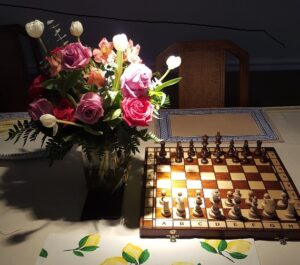
\includegraphics[width=.3\textwidth]{FlowersAndChess-300x265.jpg}
\end{wrapfigure}

There was a time in my youth when I was fascinated by the Shaman Don Juan. I did not necessarily believe the accounts about him (facts/events), yet his teachings reached into my soul. I had forgotten about him until a few days ago when I did a search for some quotes. I was amazed at how much I had retained even if, at this point in life, I had forgotten the source. This is fundamental:

\begin{quotex}
The basic difference between an ordinary man and a warrior is that a warrior takes everything as a challenge while an ordinary man takes everything as a blessing or a curse.
\end{quotex}


You see, the ordinary man is passive. Things just happen to him and his emotions fluctuate accordingly. The warrior, on the other hand, has a goal, a destiny. He expects challenges and obstacles along the way. Yet he is also blessed by those who aid and love him. He is confident because his life is ultimately guided by Providence.

\paragraph{Unmanifested Possibilities}


\begin{quotex}
The threat is stronger than the execution.
\flright{\textsc{Aron Nimzowitsch}}
\end{quotex}

When I was a boy, I loved chess. My father had given me a folding chess board and some wooden pieces in a crumpled brown paper bag; he must have kept the same bag since university. He taught me the game, but stopped playing with me after I began to beat him.

Besides playing, and beating the neighborhood boys while blindfolded, I was a great student of chess. I would devour chess books and replay the most famous games. After learning the fundamentals, I discovered the rebel Aron Nimzowitsch. His commentaries excited me. Aspects of his system are valuable to the warriors: controlling the center, overprotection of important pieces, blockades, prophylaxis. I could never forget the desperado piece since I have been a desperado. His system: `first restrain, then blockade and finally destroy'. Good advice.

An essential aspect of chess analysis is to follow up on the moves not taken. So the reader does not blindly replay the actual game; he must, in addition, play out all the alternative moves. A joke among chess players is that the best games are the ones that were never played.

Our lives are likewise replete with unmanifested possibilities. Sometimes you need to replay them in your mind to learn of what you did well and what you did poorly. Often, memories are forced on you, either in dreams or spontaneous eruptions. Where did you apply power? What did you protect and prevent? Have you identified your friends and foes?

\textbf{Rene Guenon} insists that there is no fundamental difference between the Possible and the Real. Could that mean that there are alternative universes in which your Counterpart made a different choice? I don't think so. A warrior has one chance; he must make the choice when it presents itself to him. Rather, our unmanifested possibilities are just as much a part of our personalities as those that are manifested.

\paragraph{The Path Taken}


\begin{quotex}
A man of knowledge lives by acting, not by thinking about acting.
\end{quotex}


I had a fb friend several years ago named Joe. He was a supercorrect Catholic and libertarian, always eager to engage in arguments. He thought he could use an argument to compel someone to accept his point of view. He unfriended me as unequal to his intellect.

He did not understand that the greatest gift to the human being is freedom. As \textbf{Arthur Schopenhauer} pointed out in \emph{On the Fourfold Root of the Principle of Sufficient Reason}, logic has its own compulsion. That is why it cannot be ultimate. Otherwise, your robots and even your sexbot would reason themselves to faith.

Recently, I encountered him again. He had become a depressed nihilist who had lost his faith. He did not see intellectual nihilism as liberation, for now he could choose his own path without the burden of his supercilious arguments.

When I myself had reached that point, I felt free to choose my own way, to manifest my own possibilities, my personal \textbf{Path with a Heart}. I resolved to live a Life based on High Culture, an ascetic lifestyle, and the quest for scientific knowledge.

My guideposts were the greatness that was Greece, the grandeur that was Rome, the secret gnosis of ancient Egypt, and the lofty metaphysics of the High Middle Ages.

The True, the Good, the Beautiful, are the stars that light the night sky for me. The goal is Love. That is a Path with a Heart.

Whenever I fail, I become a desperado, somehow finding victory out of apparent failure.


\flrightit{Posted on 2022-05-25 by Cologero}

\begin{center}* * *\end{center}

\begin{footnotesize}
\begin{sffamily}
\texttt{Michael M on 2022-05-26 at 09:47 said:}

To realize a path chosen is not in alignment with the heart can be agonizing as the pressures work against man to keep him there (General Law) and his own illusions, false duties etc. The absolute nature of the `I' in a path of the heart cannot be debated or argued, only lived joyously and suffered through, there lies a terrible and beautiful type of destiny.

\hfill

\texttt{Juan Martinez on 2022-05-29 at 23:31 said:}

``My guideposts were the greatness that was Greece, the grandeur that was Rome, the secret gnosis of ancient Egypt, and the lofty metaphysics of the High Middle Ages.

The True, the Good, the Beautiful, are the stars that light the night sky for me. The goal is Love. That is a Path with a Heart.''

This is well put. Thank you. I am learning much from your site and from the commenters, et al..

\hfill

\texttt{Juliano on 2026-04-22 at 16:31 said:}

I have read this text many times. One of my favorites. Thank you Mr Charles.

\end{sffamily}
\end{footnotesize}

